\begin{figure}[H]
    \centering
    %% Creator: Inkscape 1.0.2 (e86c870879, 2021-01-15, custom), www.inkscape.org
%% PDF/EPS/PS + LaTeX output extension by Johan Engelen, 2010
%% Accompanies image file '21_grafo.pdf' (pdf, eps, ps)
%%
%% To include the image in your LaTeX document, write
%%   \input{<filename>.pdf_tex}
%%  instead of
%%   \includegraphics{<filename>.pdf}
%% To scale the image, write
%%   \def\svgwidth{<desired width>}
%%   \input{<filename>.pdf_tex}
%%  instead of
%%   \includegraphics[width=<desired width>]{<filename>.pdf}
%%
%% Images with a different path to the parent latex file can
%% be accessed with the `import' package (which may need to be
%% installed) using
%%   \usepackage{import}
%% in the preamble, and then including the image with
%%   \import{<path to file>}{<filename>.pdf_tex}
%% Alternatively, one can specify
%%   \graphicspath{{<path to file>/}}
%%
%% For more information, please see info/svg-inkscape on CTAN:
%%   http://tug.ctan.org/tex-archive/info/svg-inkscape
%%
\begingroup%
  \makeatletter%
  \providecommand\color[2][]{%
    \errmessage{(Inkscape) Color is used for the text in Inkscape, but the package 'color.sty' is not loaded}%
    \renewcommand\color[2][]{}%
  }%
  \providecommand\transparent[1]{%
    \errmessage{(Inkscape) Transparency is used (non-zero) for the text in Inkscape, but the package 'transparent.sty' is not loaded}%
    \renewcommand\transparent[1]{}%
  }%
  \providecommand\rotatebox[2]{#2}%
  \newcommand*\fsize{\dimexpr\f@size pt\relax}%
  \newcommand*\lineheight[1]{\fontsize{\fsize}{#1\fsize}\selectfont}%
  \ifx\svgwidth\undefined%
    \setlength{\unitlength}{460.22099304bp}%
    \ifx\svgscale\undefined%
      \relax%
    \else%
      \setlength{\unitlength}{\unitlength * \real{\svgscale}}%
    \fi%
  \else%
    \setlength{\unitlength}{\svgwidth}%
  \fi%
  \global\let\svgwidth\undefined%
  \global\let\svgscale\undefined%
  \makeatother%
  \begin{picture}(1,0.19870508)%
    \lineheight{1}%
    \setlength\tabcolsep{0pt}%
    \put(0,0){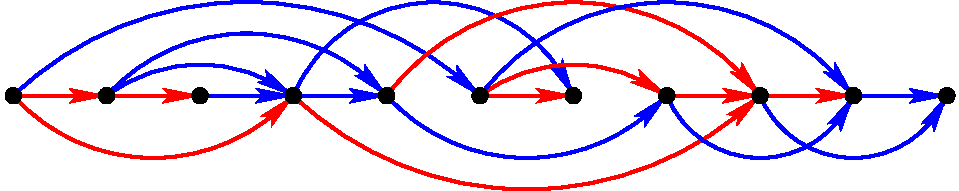
\includegraphics[width=\unitlength,page=1]{respostas/21_grafo.pdf}}%
    \put(0.98846278,0.06679875){\color[rgb]{0,0,0}\makebox(0,0)[lt]{\lineheight{1.25}\smash{\begin{tabular}[t]{l}$z$\end{tabular}}}}%
    \put(-0.0020552,0.06702944){\color[rgb]{0,0,0}\makebox(0,0)[lt]{\lineheight{1.25}\smash{\begin{tabular}[t]{l}$p$\end{tabular}}}}%
    \put(0.09591444,0.06701983){\color[rgb]{0,0,0}\makebox(0,0)[lt]{\lineheight{1.25}\smash{\begin{tabular}[t]{l}$q$\end{tabular}}}}%
    \put(0.19245584,0.06686864){\color[rgb]{0,0,0}\makebox(0,0)[lt]{\lineheight{1.25}\smash{\begin{tabular}[t]{l}$r$\end{tabular}}}}%
    \put(0.29154197,0.05085898){\color[rgb]{0,0,0}\makebox(0,0)[lt]{\lineheight{1.25}\smash{\begin{tabular}[t]{l}$s$\end{tabular}}}}%
    \put(0.38770429,0.06722658){\color[rgb]{0,0,0}\makebox(0,0)[lt]{\lineheight{1.25}\smash{\begin{tabular}[t]{l}$t$\end{tabular}}}}%
    \put(0.48495918,0.06684231){\color[rgb]{0,0,0}\makebox(0,0)[lt]{\lineheight{1.25}\smash{\begin{tabular}[t]{l}$u$\end{tabular}}}}%
    \put(0.58256316,0.06709827){\color[rgb]{0,0,0}\makebox(0,0)[lt]{\lineheight{1.25}\smash{\begin{tabular}[t]{l}$v$\end{tabular}}}}%
    \put(0.68017119,0.05058472){\color[rgb]{0,0,0}\makebox(0,0)[lt]{\lineheight{1.25}\smash{\begin{tabular}[t]{l}$w$\end{tabular}}}}%
    \put(0.77719442,0.05044547){\color[rgb]{0,0,0}\makebox(0,0)[lt]{\lineheight{1.25}\smash{\begin{tabular}[t]{l}$x$\end{tabular}}}}%
    \put(0.89065104,0.06694284){\color[rgb]{0,0,0}\makebox(0,0)[lt]{\lineheight{1.25}\smash{\begin{tabular}[t]{l}$y$\end{tabular}}}}%
  \end{picture}%
\endgroup%


    \caption{Para quem tem dificuldades de distinguir as cores, as arestas vermelhas são: $(p, q)$, $(q, r)$, $(p, s)$, $(s, x)$, $(t, x)$, $(u, v)$, $(u, w)$, $(w, x)$ e $(x, y)$. Caminhos de comprimento zero ou um são sempre válidos. Os caminhos $(q, s, t, x, z)$ e $(p, s, t, w, y)$ também são válidos. Já o caminho $(p, q, s, t, x, y, z)$ não é válido pois $(t, x)$ e $(x, y)$ são arestas consecutivas de cor vermelha neste caminho.}
\end{figure}

\subsection{a} Para cada vértice $i$ do grafo acima, indique os valores $azul[i]$ e $verm[i]$ (alguns valores estão preenchidos).

\itemdsep[0.25]
